\documentclass[../main.tex]{subfiles}

\begin{document}
    
\chapter{Introduction}

The United States today is home to approximately 20,000 publicly traded corporations. Despite only a small minority capturing the public eye on a regular basis, they all contribute to the foundation on which the modern Global economy is built. As postulated by nearly all economic theory, the efficient flow of capital and information through these markets is necessary for a healthy economy.

To this end, market sectors and the practice of sectorization have been an integral component of healthy markets, both in the United States and around the world. Market Sectors - in their ideal form - group together corporations of similar business function and economic operating arena for easier regulation, management, investment, etc. A related practice to that of market sectorization is Market Segmentation, the practice of dividing a market into subgroups of consumers (i.e. \textit{segments}).

The evolution of Market Segments and Market Sectors have historically been extremely useful metrics for gauging the development of the economy. There are four generally accepted stages of evolution in market segmentation; fragmentation, unification, segmentation, and hyper-segmentation.\citeFormat{\cite{Tedlow1996NewAmerica}} The United States economy - being the archetype on which this four-stage heuristic was built - developed through these four stages over the course of the last two centuries. Being a decidedly \textit{hyper-segmented} market today, there is a marked shift toward ever more narrow market segments. This shift has notably been amplified by the enablement of hyper-targeted marketing and product delivery by technologies such as the smartphone.

\section{Applications of Market Sectors}

In addition to being a useful theoretical guideline for the stage of growth of an economy, market sectors and segments also serve extremely valuable functional roles in the modern economy.

The Securities and Exchange Commission (SEC) of the United States classifies every company into a sepecific sector, as a part of its regulatory perogative.\citeFormat{\cite{U.S.SecuritiesandExchangeCommission2019DivisionList}} This is a key prerequisite to effective monitoring and governance. The sheer scope of the modern economy guarantees the necessity of such classificaitons; the current scope of the economy spans - indisputably - all facets of Human culture. This gargantuan scope demands specialization, which - in turn - demands organization; motivating the need for market sectors.

Credit rating is the practice of evaluating the risk of a prospective counterparty in a transaciton. This metric is integral to risk management, ånd relies on evaluating the probability that a candidate counterparty to a transaction will not default on their obligation. In addition to the idiosyncratic forces affecting any given corporation, its risks are often decomposed to market factors and - increasingly - market sector factors. This means that a positive outlook on a specific market sector would imply a more positive outlook for the consituent corporations composing that sector, underscoring the importance of appropriate and accurate sector assignment. The significance of accurate sector assignments is reaffirmed by the fact that all of the \textit{Big 3} credit rating agencies cite market sector rating as a key component in determining credit ratings.\citeFormat{\cite{StandardPoorsRatingServices2014CorporateMethodology}}\citeFormat{\cite{Hill2016FinancialMethodology}}\citeFormat{\cite{FitchRatings2019ProceduresRatings}}

Finally, another major application of asset sectors is to provide investors with targeted exposure to specific segments of hte the market. It is a well-known corollary of Modern Portfolio Theory that diversification provides savings an enhanced risk-return portfolio for any given basket of assets.\citeFormat{\cite{Markowitz1952PortfolioSelection}} This, combined with the excellent cost savings provided by modern Exchange Traded Funds (hereafter \textit{ETFs}), has led to a rapid prolification of these products in the Financial System today.

\section{Status Quo}

In the United States today, there are myriad sectorization taxonomies (hereafter \textit{sector universes}). To limit the scope of this analysis, we will focus on two of the three most popular sector classification systems\citeFormat{\cite{FidelityInvestments2019KnowIndustries}}; the GICS, and the ICB.

\subsection{GICS - Global Industry Classification Standard}

\begin{wrapfigure}[12]{r}{0.3\textwidth}
    \centering
    \vspace{\wrapfigadjustment}
    \fbox{
    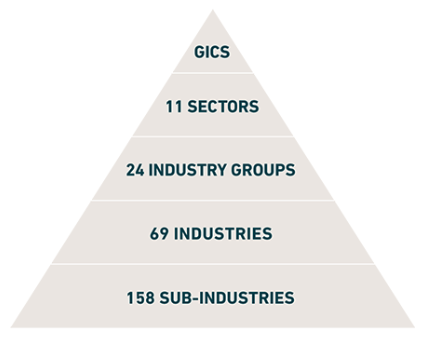
\includegraphics[width=.9\linewidth]{images/msci_gics_breakdown.png}
    }
    \caption{Overview of the GICS Sector Universe}
    \label{fig:introduction:gics_breakdown}
\end{wrapfigure}

The GICS (Global Industry Classification Standard)\citeFormat{\cite{MSCI-MorganStanleyCapitalInternational2019GICSMSCI}} is published by MSCI (Morgan Stanley Capital International) and S\&P (Standard \& Poor's). This classification is arguably the most widely used sector universe in the United States, and provides the basis for the poular S\&P 500 Market Sectors and Market Sector ETFs used in popular financial analysis resources.

Corporations are divided into four different categories, each in increasing order of specificity. The first classification is its \textit{sector} (the most general), followed by the \textit{industry group}, \textit{industry}, and finally \textit{sub-industry}, the most specific. The hierarchical taxonomy of these sector classifications are displayed in Figure~\ref{fig:introduction:gics_breakdown}\citeFormat{\cite{MSCI-MorganStanleyCapitalInternational2019GICSMSCI}}.

Additionally, the GICS methodology specification indicates that sector assignments and assignment updates are made primarily based on three factors; the primary source of revenue, earnings and market perception, and finally - in the case of a new company - information derived from the company prospectus.\citeFormat{\cite{SPGlobalMarketIntelligence2018GlobalMethodology}}

\textit{Note:} A key change in this sector classification taxonomy was made in the Fall of last year (September 2018).\citeFormat{\cite{MSCIResearch2018ConsultationIndexes}} Specifically, the previously-labeled \textit{Telecommunications Services} sector was broadened and renamed to \textit{Communication Services}. Company sector assignment changes were also made commensurate to the name and scope change:

\begin{itemize}
    \item Media companies were moved from \textit{Consumer Discretionary} to \textit{Communication Services}
    \item Internet services comapnies were moved from \textit{Information Technology} to \textit{Communication Services}
    \item E-Commerce companies were moved from \textit{Information Technology} to \textit{Consumer Discretionary}
\end{itemize}

\subsection{ICB - Industry Classification Benchmark}

The ICB (Industry Classification Benchmark)\citeFormat{\cite{FTSEInternationalLimited2019IndustryRussell}} is published by FTSE International (previously jointly owned by Dow Jones and FTSE). Similarly to the GICS, the ICB also classifies corporations into four increasingly specific categories; \textit{industry} (the most general), \textit{supersector}, \textit{sector}, and finally \textit{subsector}, the most specific. A visualization of the ICB taxonomy is reproduced in Figure~\ref{fig:introduction:icb_breakdown}\citeFormat{\cite{FTSEInternationalLimited2019IndustryRussell}}.


Similar to the GICS, ICB too utilizes three main criteria when classifying companies into specific sectors, and other cateogries. They are; the primary source of revenue, description in annual filings, and - in the case of a new company - information derived from the company prospectus, or regulatory filing descriptions (company-supplied).


\section{Key Limitations}

\begin{wrapfigure}[11]{R}{0.3\textwidth}
    \centering
    \vspace{\wrapfigadjustment}
    \fbox{
    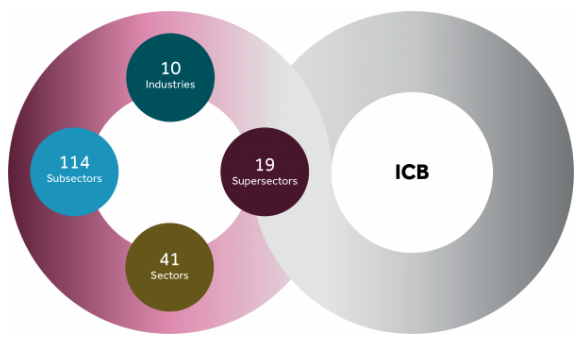
\includegraphics[width=.9\linewidth]{images/ftse_icb_breakdown.png}
    }
    \caption{Overview of the MSCI Sector Universe}
    \label{fig:introduction:icb_breakdown}
\end{wrapfigure}

In this section, we analyze the GICS and ICB sector classification schemes described above through the lens of their limitations. We then utilize these key limitations to inform our research goals.

As discussed above, both GICS and ICB utilize information from company prospectuses to determine an initial sector assignment. Unfortunately, this inherently implies that the initial classification is not based on an objective criteria, and is highly subject to the initial vision of the authors of the company prospectus. This is in stark contrast to utilizing a company-specific quantifiable metric, and relies on accurate reporting in the initial prospectus; a document whose authors are highly incentivized to inflate in grandiosity.

Furthermore, the initial sector groups and constituent sectors in both classification schemes are defined based on a qualitative analysis of the economy, as opposed to a quantitatively-driven process. Similarly, the number of sectors in the market is also aribtrary, and not based on a quantifiable or objective metric.

Additionally, as implied by the reorganization of the GICS classification scheme in 2018, there appears to be no stong objective criteria governing the creation and deletion of new sectors. The companies reassigned during this reorganization were not new, and imply that the underlying newly created sector existed before its recognition by the GICS scheme.

As evidenced by the short list of limitations outlined in this section, the status quo of market sector classificaitons are far from perfect. To this end, we hope to develop a new \textit{Learned Sectors} scheme, addressing each of the limitations described above.

\end{document}